Pooling is a way of shrinking the non-channel dimension of some input. The idea of pooling reminds a lot about how convolution works. Pooling also operates with a kernel, sliding over the features. Two popular pooling methods are Max-pooling and Average-pooling. In pooling methods, we have a kernel of some predefined size. This kernel will slide over the features, just like how the filter traveled through the features, during a convolution. \\

\noindent
The output of Max-pooling (figure 7), will always take the maximum value, of the features where the kernel is currently at. The output of Average-pooling (figure 8), will take the average of the features where the kernel is currently at. \\


\begin{figure}[!ht]
  \centering
  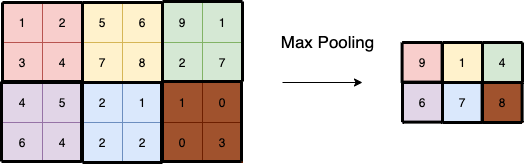
\includegraphics[scale=0.4]{latex/IMGs/maxpooling.png}
  \caption{2x2 kernel, max-pool}\label{Baseline:before}
\end{figure}

\noindent
Defining the values within the striding kernel with size $h$x$w$ as $A$, the function looks like:
$$
Maxpool(A) = max(0,A)
$$

\begin{figure}[!ht]
  \centering
  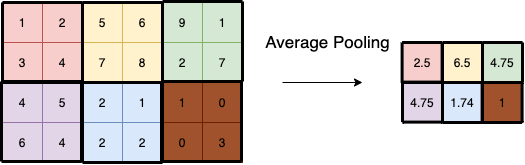
\includegraphics[scale=0.4]{latex/IMGs/averagepooling.png}
  \caption{2x2 kernel, average-pool}\label{Baseline:before}
\end{figure}

\noindent
Defining the values within the striding kernel with size $h$x$w$ as $A$, the function looks like:

$$
Averagepool(A) = \frac{\sum_{i \in A} A_i}{h * b}
$$




